\begin{figure}[h]
    \centering
    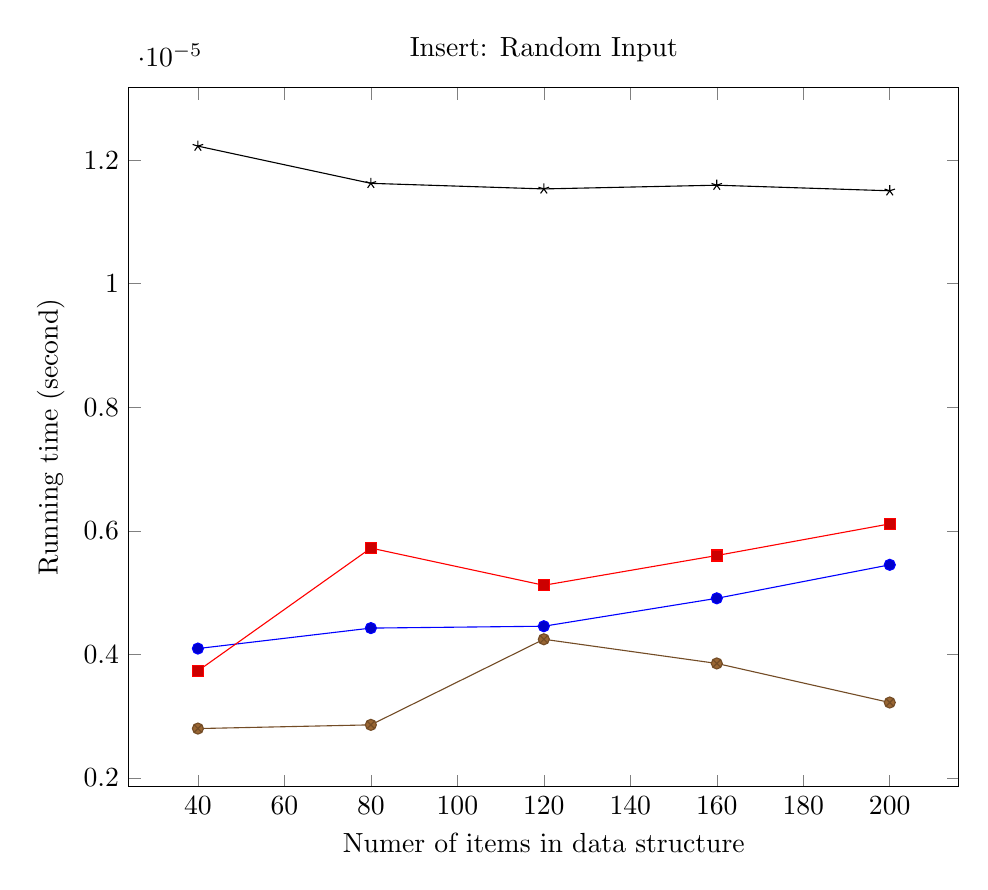
\begin{tikzpicture}
        \begin{axis}[
            xlabel={Numer of items in data structure},
            ylabel={Running time (second)},
            title={Insert: Random Input},
            width=\textwidth
        ]
		\addplot coordinates {
			(200, 5.451273595205586e-06)
			(160, 4.9091579890525596e-06)
			(120, 4.4573949839255e-06)
			(80, 4.427277450250178e-06)
			(40, 4.0959845798216324e-06)
		};
		\addplot coordinates {
			(200, 6.113859336058514e-06)
			(160, 5.601861263582197e-06)
			(120, 5.119980724778428e-06)
			(80, 5.722331398282099e-06)
			(40, 3.73457417572054e-06)
		};
		\addplot coordinates {
			(200, 3.2225761032428356e-06)
			(160, 3.855044310421829e-06)
			(120, 4.2465722481996315e-06)
			(80, 2.8611656991417433e-06)
			(40, 2.8009306317910987e-06)
		};
		\addplot coordinates {
			(200, 1.1504897863913454e-05)
			(160, 1.1595250464939421e-05)
			(120, 1.1535015397590165e-05)
			(80, 1.1625367998614743e-05)
			(40, 1.2227718672118415e-05)
		};
        \legend{}
        \end{axis}
    \end{tikzpicture}
    \caption{Average of 0 operations, benchmarked every 0, starting at 0.}
\end{figure}